
\documentclass[conference]{IEEEtran}
% If the IEEEtran.cls has not been installed into the LaTeX system files, manually specify the path to it: e.g., \documentclass[conference]{../sty/IEEEtran} 

\usepackage{graphicx, times, amsmath} 

\hyphenation{op-tical net-works semi-conduc-tor IEEEtran}

\IEEEoverridecommandlockouts	

\providecommand{\keywords}[1]{\textbf{\textit{Index terms---}} #1}

\begin{document}

\title{\ \\ \LARGE\bf Semtiment Analysis on Movie Reviews Using Machine Learning Classifiers Report \thanks{Zeeshan Ahmed. 
School of Computer Science and Technology, Beijing Institute of Technology
(email: shancstm@yahoo.com).}
\thanks{Haq Ijaz Ul. 
School of Computer Science and Technology, Beijing Institute of Technology
(engr.ijaz@outlook.com).}
\thanks{David Matthew. 
School of Computer Science and Technology, Beijing Institute of Technology
(chen7david@me.com).}
}

\author{Zeeshan Ahmed, Haq Ijaz Ul and David Matthew}

%\specialpapernotice{(Datamining Report Paper)}

% make the title area\maketitle
\maketitle

\begin{abstract}

Sentiment analysis has a huge number of applications in automated systems. Sentiment analysis is a part of natural language processing that deals with the analysis of the opinion and subjectivity in a text. In this report paper we will study the results of applying support vector machine classifier for sentiment analysis of user opinion of movies expressed through reviews over IMDb movies database. The goal is to develop a classifier that categorizes sentiment of each review of movies as being positive or negative. The results suggests that the classifier obtains an accuracy of over 58\% on the reviews dataset.

\end{abstract}

\keywords{ Opining mining, Sentiment classification, Support Vector Machines }


\section{Introduction}

Sentiment Analysis is defined as the process to determine the attitude of a speaker or a writer with respect to some topic. Recently, it has become an active research topic, mostly due to its potential use and importance in a wide spectrum of applications of popularity analysis to product user satisfaction analysis. With the rapid growth of online information, a huge amount of data is available for the sentiment analysis. However, the sheer volume of information is a challenge itself. To separate relevant information from the irrelevant, and to gain knowledge from this unprecedented volume of huge data, an automatic analysis method is essential.

In this project, we use the support vector machine, a supervised machine learning algorithm in learning
sentiment classifier and test the effectiveness of the classification model to predict the sentiment of the test dataset.


\section{Approach}

\subsubsection{Input Data}

The input data for the sentiment analysis comes from the Internet Movie Database (IMDb): a collection of movie reviews \cite{IMDB}. The datasets containing the feature vectors of the movie reviews are obtained from a sentiment research study \cite{ARPDAC11}. One labeled training dataset and one labeled testing dataset form the input datasets for our evaluation. The dataset contains 50,000 reviews split into 25,000 train and 25,000 test reviews vectors. The overall distribution of labels is balanced (25,000 positive and 25,000 negative). At most 30 reviews are involved for any given movie because reviews for the same movie tend to have correlated ratings. The train and test sets contain a disjoint set of movies. In the labeled train/test sets, a negative review has a score <= 4 out of 10, and a positive review has a score >= 7 out of 10. Thus reviews with more neutral ratings are not included in the train/test sets.

\subsubsection{Feature Extraction}

For text analysis, one standard feature extraction approach is to represent text phrases as n-grams, using the sequences of n words. The feature vectors thus produced span a high dimensional feature space and hence is expected to be very sparse. The special nature may cause deterministic machine learning algorithms to "overfit".

\subsubsection{Data Modeling}

Since machine learning classifiers cannot handle raw text data, the text reviews are converted
into feature vectors which is a compact representation that consists of all unique word features. Each
review is represented as vector of the words, one attribute per word position. The mapping process is
applied to both the train and test reviews in the corpus. All the non-word characters for instance the
punctuations used in the reviews are removed from the feature space.

Each instance of the modeled movie review vector for the classifier comprises of two main parts:
sentiment class and feature vector. We represent the class part of the vector as +1 for positive review
and -1 for a negative review. The second feature vectors part contains the every word feature that
occurred in the review paired with the number of times it occurs in that review.


\section{SVM}

Support Vector Machine (SVM) classifier separates two classes by a function, which it learns
from the training examples. The goal of SVM is to find an optimal separating hyperplane that
maximizes the separation distance between the hyperplane and the nearest data point of each class. For
a set of training example feature vectors ${v1, v2, ... vn }$ each vector belonging to one of the two
classes, a hyperplane is generated to separate the two classes given by:

$(w, x) + b = 0$

The set of vectors given by the above equation is optimally separated by the hyperplane if it is
separated without error and the distance between the closest vector to the hyper plane is maximal.
By computing the hyper plain of a given set of training review examples, the support vector machine
builds a classification model to predict which category a new review falls into.


%\begin{figure}

%\title{SVM support vectors}
%\caption{Learning support vector classifiers.}
%\end{figure}

\begin{figure*}
\centerline{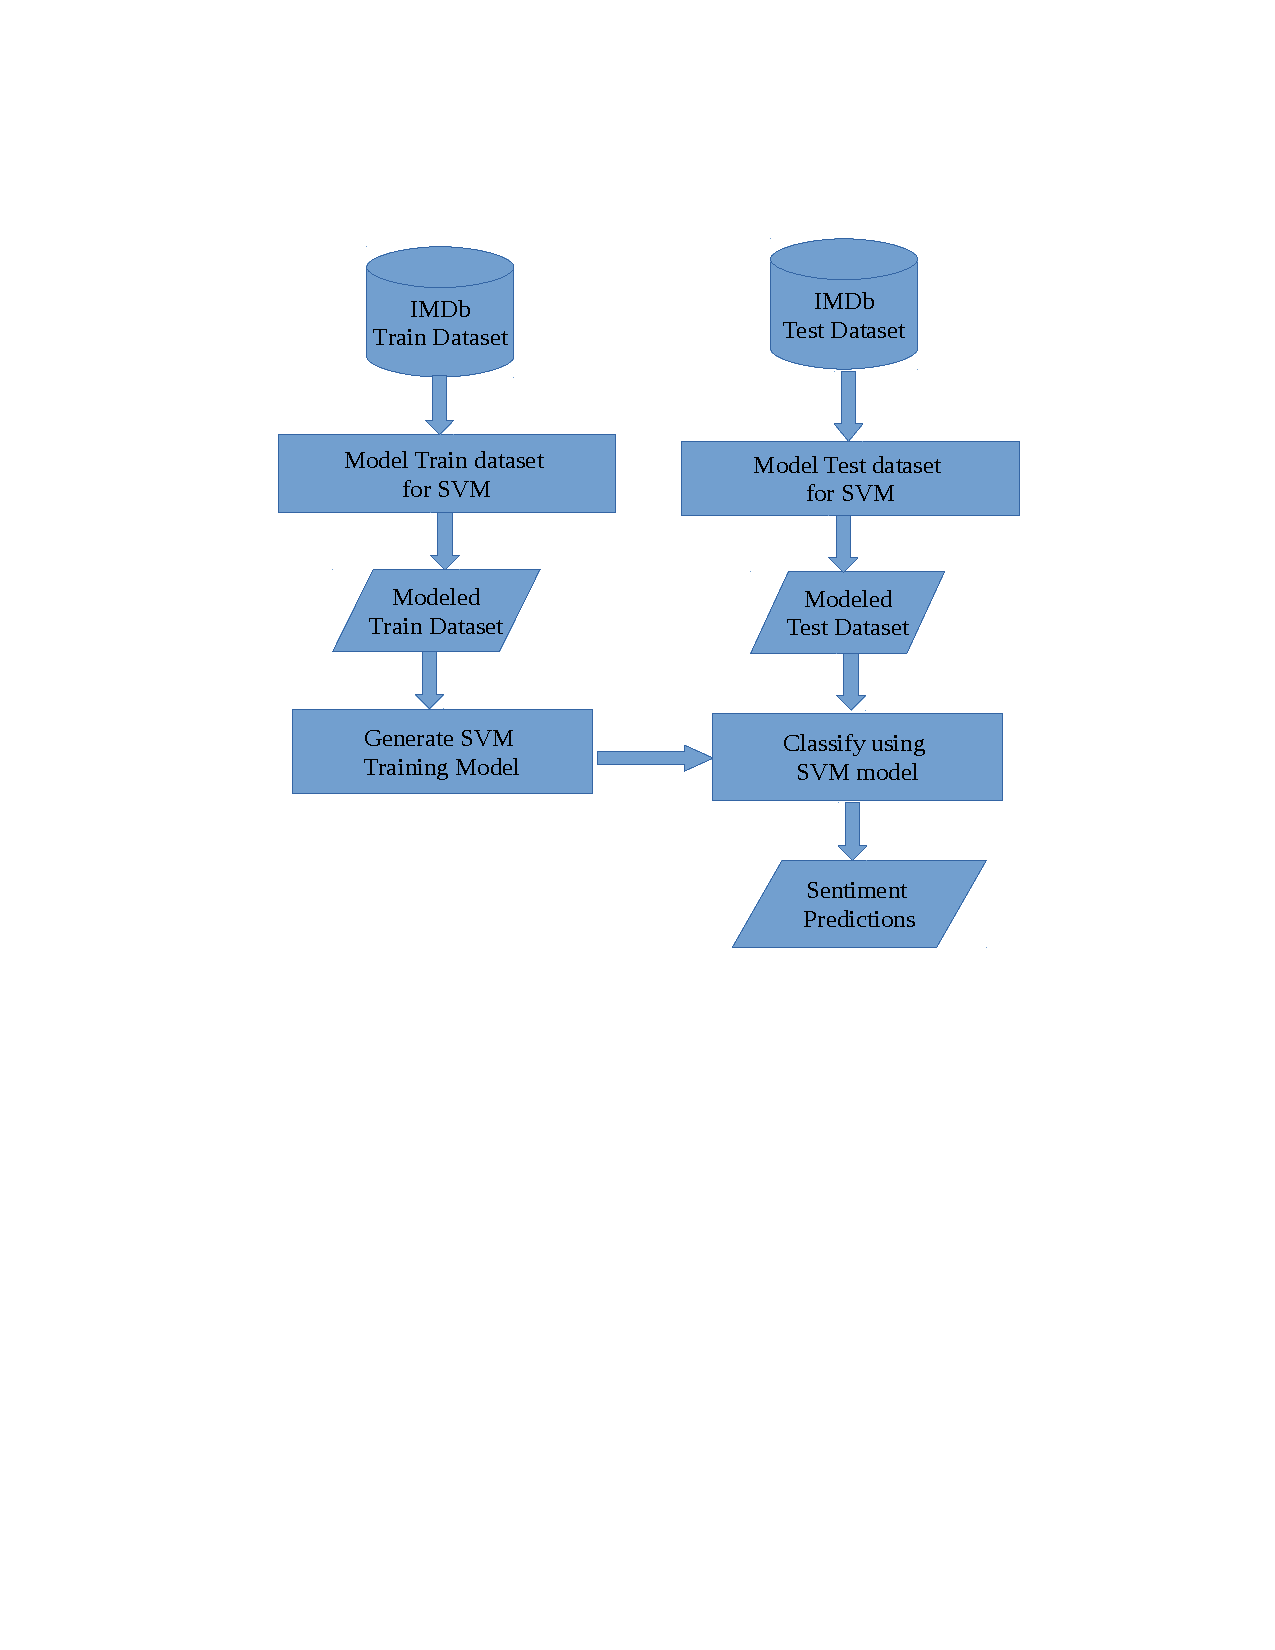
\includegraphics[scale=0.6]{Implementation.pdf}}
\caption{Sentiment Prediction approach of Movie Reviews}
\label{fig:approach}
\end{figure*}


\begin{center}
\begin{figure*}[ht]
\centerline{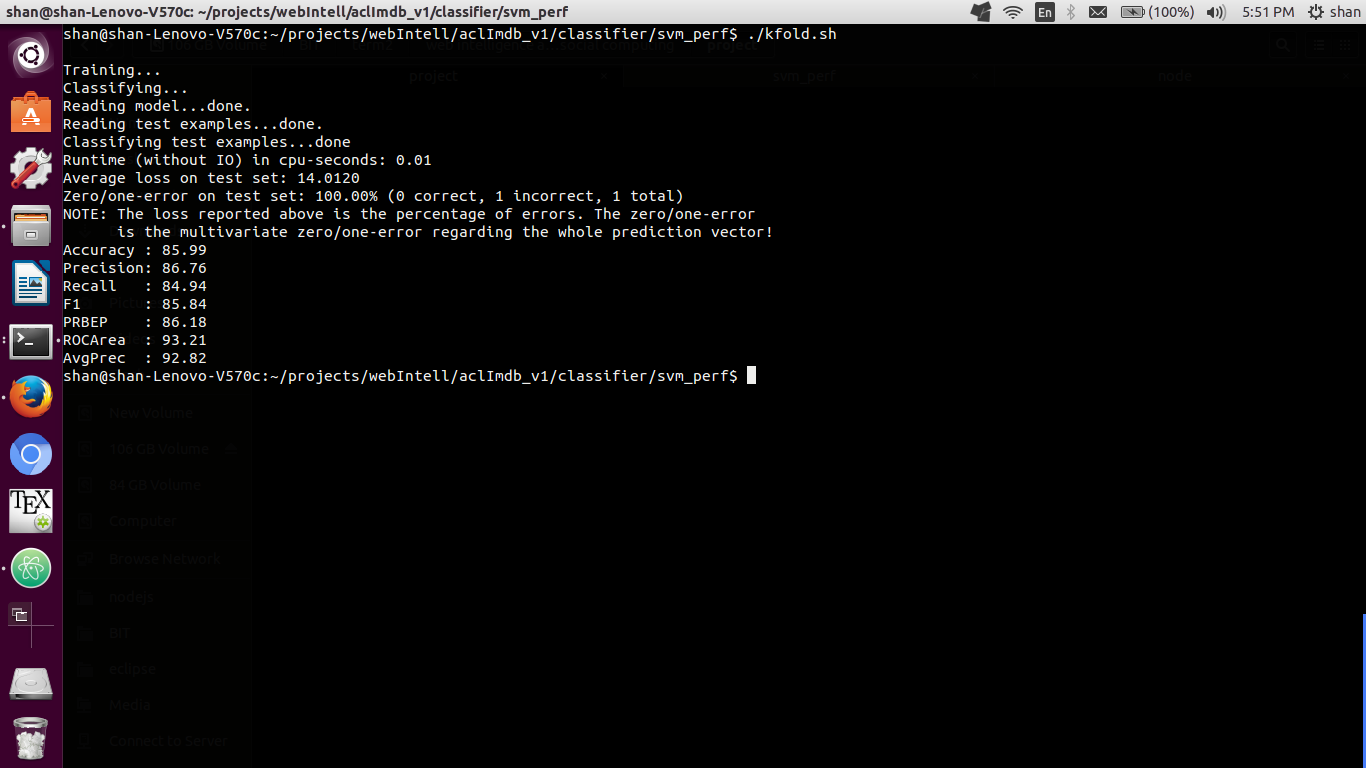
\includegraphics[scale=0.3]{SentimentAnalysisSVM.png}}
\caption{Support Vector Machine performance}
\label{fig:SVMperformance}
\end{figure*}    
\end{center}

There are many different possible hyperplanes separating the two classes and one optimal hyperplane.
The crosses and circles represent positive and negative classes in training vectors, respectively, while
the lines represent decision surfaces or the hyperplanes. Decision surface plane σi shown as the thicker
line is the most optimal separator. It is the middle element of the widest set of parallel decision
surfaces. In other words its minimum distance to any training example vector is maximum. Small
boxes indicate the support vectors.

SVM attempts to find, among all the surfaces $σ1 , σ2 , . . .$ in T-dimensional space that separate the
positive from the negative training examples (decision surfaces), the σi that separates the positives
from the negatives by the widest possible margin, that is, such that the separation property is invariant with respect to the widest possible translation of $σi$. SVM chooses the middle element from the set in which the maximum distance between two elements in the highest. This most optimal decision surface or hyperplane is determined by only a small set of training examples, called the support vectors. The method is also applicable in the case of positives and the negatives which are not linearly separable.


\section{Implementation}

Figure~\ref{fig:approach} summarizes the sentiment analysis and prediction process. We used the C implementation of the SVM classifier called SVM light \cite{SVMlight} to predict the sentiment of movie comments. SVM light is an implementation of Vapnik's Support Vector Machine \cite{V95} for the problem of pattern recognition, regression, and learning a ranking function. The algorithm has scalable memory requirements and can handle problems with many thousands of support vectors efficiently.

We trained the support vector machine classifier implementation, SVM light with the linear kernel
function. The classifier implementation can process hundred thousands of training and handle some
thousands of support vectors. The parameter c value of 20.0 is used in the classifier training. This parameter is the trade-off between training error and the support vector margin.


\subsection{Modifying the Feature Vectors}

We wrote the \emph{modifyVectorsSVM.js} , a Nodejs script to modify the train and test reports feature
vectors from the IMDb data according to the SVM classifier input requirement. The script uses an input
file name of the already modeled dataset with different rating values and converts them into two class
feature vectors, where each review vector becomes either a positive review or negative review instead
of the rating. The generated output is a text file with the remodeled feature vectors where the ratings are mapped into appropriate classes.

The command to execute the script when nodejs is installed is shown in the Table~\ref{table:nodejsScript}.
Note: The first feature that is the word "the" is omitted in modified feature vectors files since it occurs in all the reports and can be safely removed without affecting the classification accuracy.
The SVM classifier first trains to generate the classification model.



\begin{table} 
\centering
\caption{Nodejs script to remodel the dataset vectors for the SVM classifier}	
\begin{tabular}{c c}				
\hline \hline						
Function & Command	\\ 
\hline	
Re-model Vectors	&	node modifyVectorsSVM.js  \\ [1ex]
\hline
\end{tabular}
\label{table:nodejsScript}
\end{table}

\begin{table*} 
\centering
\caption{The SVM learn and classify functions}	
\begin{tabular}{c c}				
\hline \hline						
Function & Command	\\ 
\hline	
Learn	 &	./\verb|svm_perf_learn| -c 20 data/trainfeaturevectors.dat ./output/svmmodel.dat > /dev/null  \\
Classify &	./\verb|svm_perf_classify| data/testfeaturevectors.dat ./output/svmmodel.dat ./output/svmoutput.dat \\ [1ex]
\hline
\end{tabular}
\label{table:SVMfunctions}
\end{table*}


\subsection{Training and Sentiment Classification}


The commands to train the classifier and predict the sentiment class are shown in the Table~\ref{table:SVMfunctions}. The classifier \verb|svm_perf_learn| program takes as input the modeled feature vectors text file to generate the classification model. The \verb|svm_perf_learn| requires training vectors file name as input and the generated model file name for output. The -c switch specifies the trade-off between training error and margin.

To classify and predict the sentiment of the reviews, the \verb|svm_perf_classify| program requires the test file name and the svm model it learned in training as input and requires the classified prediction file name as it's output.        

\section{Evaluation and Results}

\subsection{Performance Metrics}



The prediction performance for the test dataset is evaluated on the performance metric of accuracy, precision and recall. Accuracy measures the proportion of all correct predictions. Precision measures the number of actual true positive predictions out of all positive predictions. Recall measures the number of true positives returned by classifier from the total number of true positive cases. The performance metrics are mathematically defined as

\begin{equation*}
Accuracy = (TP + TN) / (T P + FN + FP + T N)
\end{equation*}

\begin{equation*}
Precission = TP / (T P + FP)
\end{equation*}

\begin{equation*}
Recall = TP / (T P + FN)
\end{equation*} 

Where TP (True Positive) is the number of positive reviews predicted positive. TN (True Negative) is
the number of negative reviews, predicted correctly as negative. FN (False Negative) is the number of
positive reviews classified as negative. FP (False Positive) is the number of negative reviews predicted
as positive.
    

    
\subsection{Results}

The model trained using the SVM algorithm discussed above are evaluated on the test data set.
The total number of the reviews instances used in the classifier training is 25,000 evenly distributed as
positive and negative reviews. The dataset used for testing the classification model also has the same
number of evenly distributed instances of the reviews.

The sentiment prediction results are presented in the Figure~\ref{fig:SVMperformance}. The accuracy, precision and recall of the SVM classifier is 85.99\%, 86.76\% and 84.94\% respectively. The classifier shows better performance with the dataset. A weakness of the SVM is the imbalanced dataset in which the training examples are highly skewed towards one class while the other class only has a fewer examples. However, the dataset used in this project is balanced with equal number of training examples in each of the two sentiment classes. This improves the performance of the classifier and achieves high accuracy of over 85\%.



% use section* for appendix
%\section*{Appendix}
%Appendix contents.

% use section* for acknowledgment
\section*{Acknowledgment}
% optional entry into table of contents (if used)
%\addcontentsline{toc}{section}{Acknowledgment}
We would like to thank the IMDb reviews collectors team for providing the data for sentiment analysis.



% references section
% NOTE: BibTeX documentation can be easily obtained at:
% http://www.ctan.org/tex-archive/biblio/bibtex/contrib/doc/

% can use a bibliography generated by BibTeX as a .bbl file
% standard IEEE bibliography style from:
% http://www.ctan.org/tex-archive/macros/latex/contrib/supported/IEEEtran/testflow/bibtex
%\bibliographystyle{IEEEtran.bst}
% argument is your BibTeX string definitions and bibliography database(s)
%\bibliography{IEEEabrv,../bib/paper}
%
% <OR> manually copy in the resultant .bbl file
% set second argument of \begin to the number of references
% (used to reserve space for the reference number labels box)


%\def\V{\rm vol.~}
%\def\N{no.~}
%\def\pp{pp.~}
%\def\Pot{\it Proc. }
%\def\IJCNN{\it International Conference on Data Mining\rm }
%\def\SMC{\it IEEE Trans. Systems\rm , \it Man\rm , and \it Cybernetics\rm }

%\bibliography{SentimentAnalysis}

\begin{thebibliography}{1}

  \bibitem{IMDB} www.imdb.com.
  \bibitem{ARPDAC11} Andrew L. Maas, Raymond E. Daly, Peter T. Pham, Dan Huang, Andrew Y. Ng, and Christopher Potts. 2011. Learning word vectors for sentiment analysis. In Proceedings of the 49th Annual Meeting of the Association for Computational Linguistics: Human Language Technologies - Volume 1 (HLT '11), Vol. 1. Association for Computational Linguistics, Stroudsburg, PA, USA, 142-150.

  \bibitem{SVMlight} http://svmlight.joachims.org


  \bibitem{V95} Vladimir N. Vapnik, The Nature of Statistical Learning Theory. Springer, 1995.

\end{thebibliography}


\end{document}
